\chapter{\label{ch:results} Results and Discussion}

This chapter describes the results from the tests that were carried out during the case study as described in the previous chapter. 

\subsubsection{Generated a Normalised Distribution of Probabilities $n$-Qubit Systems}

Pure quantum state probabilities were successfully generated using the MATLAB \texttt{randn} function to return normally distributed random numbers as seen in listing \ref{lst:normally-distributed-probabilities} showing a code snippet of the \texttt{generate\_probs} function. In this study of the proposed design, the first qubit in the $n$-qubit quantum register $\ket{q_0 q_1 ... q_{n-1}}$ is the MSB and the last qubit $\ket{q_{n-1}}$ in the register is taken as the LSB. 

\subsection{Flying Qubit Transmission}

The first iteration of the quantum channel circuit was successfully implemented on breadboard using 8 red LEDs which model qubit transmission to 8 APDs represented by LDR as seen in the figure \ref{fig:quantum-channel-bread}.
\begin{figure}[!ht]
	\centering
	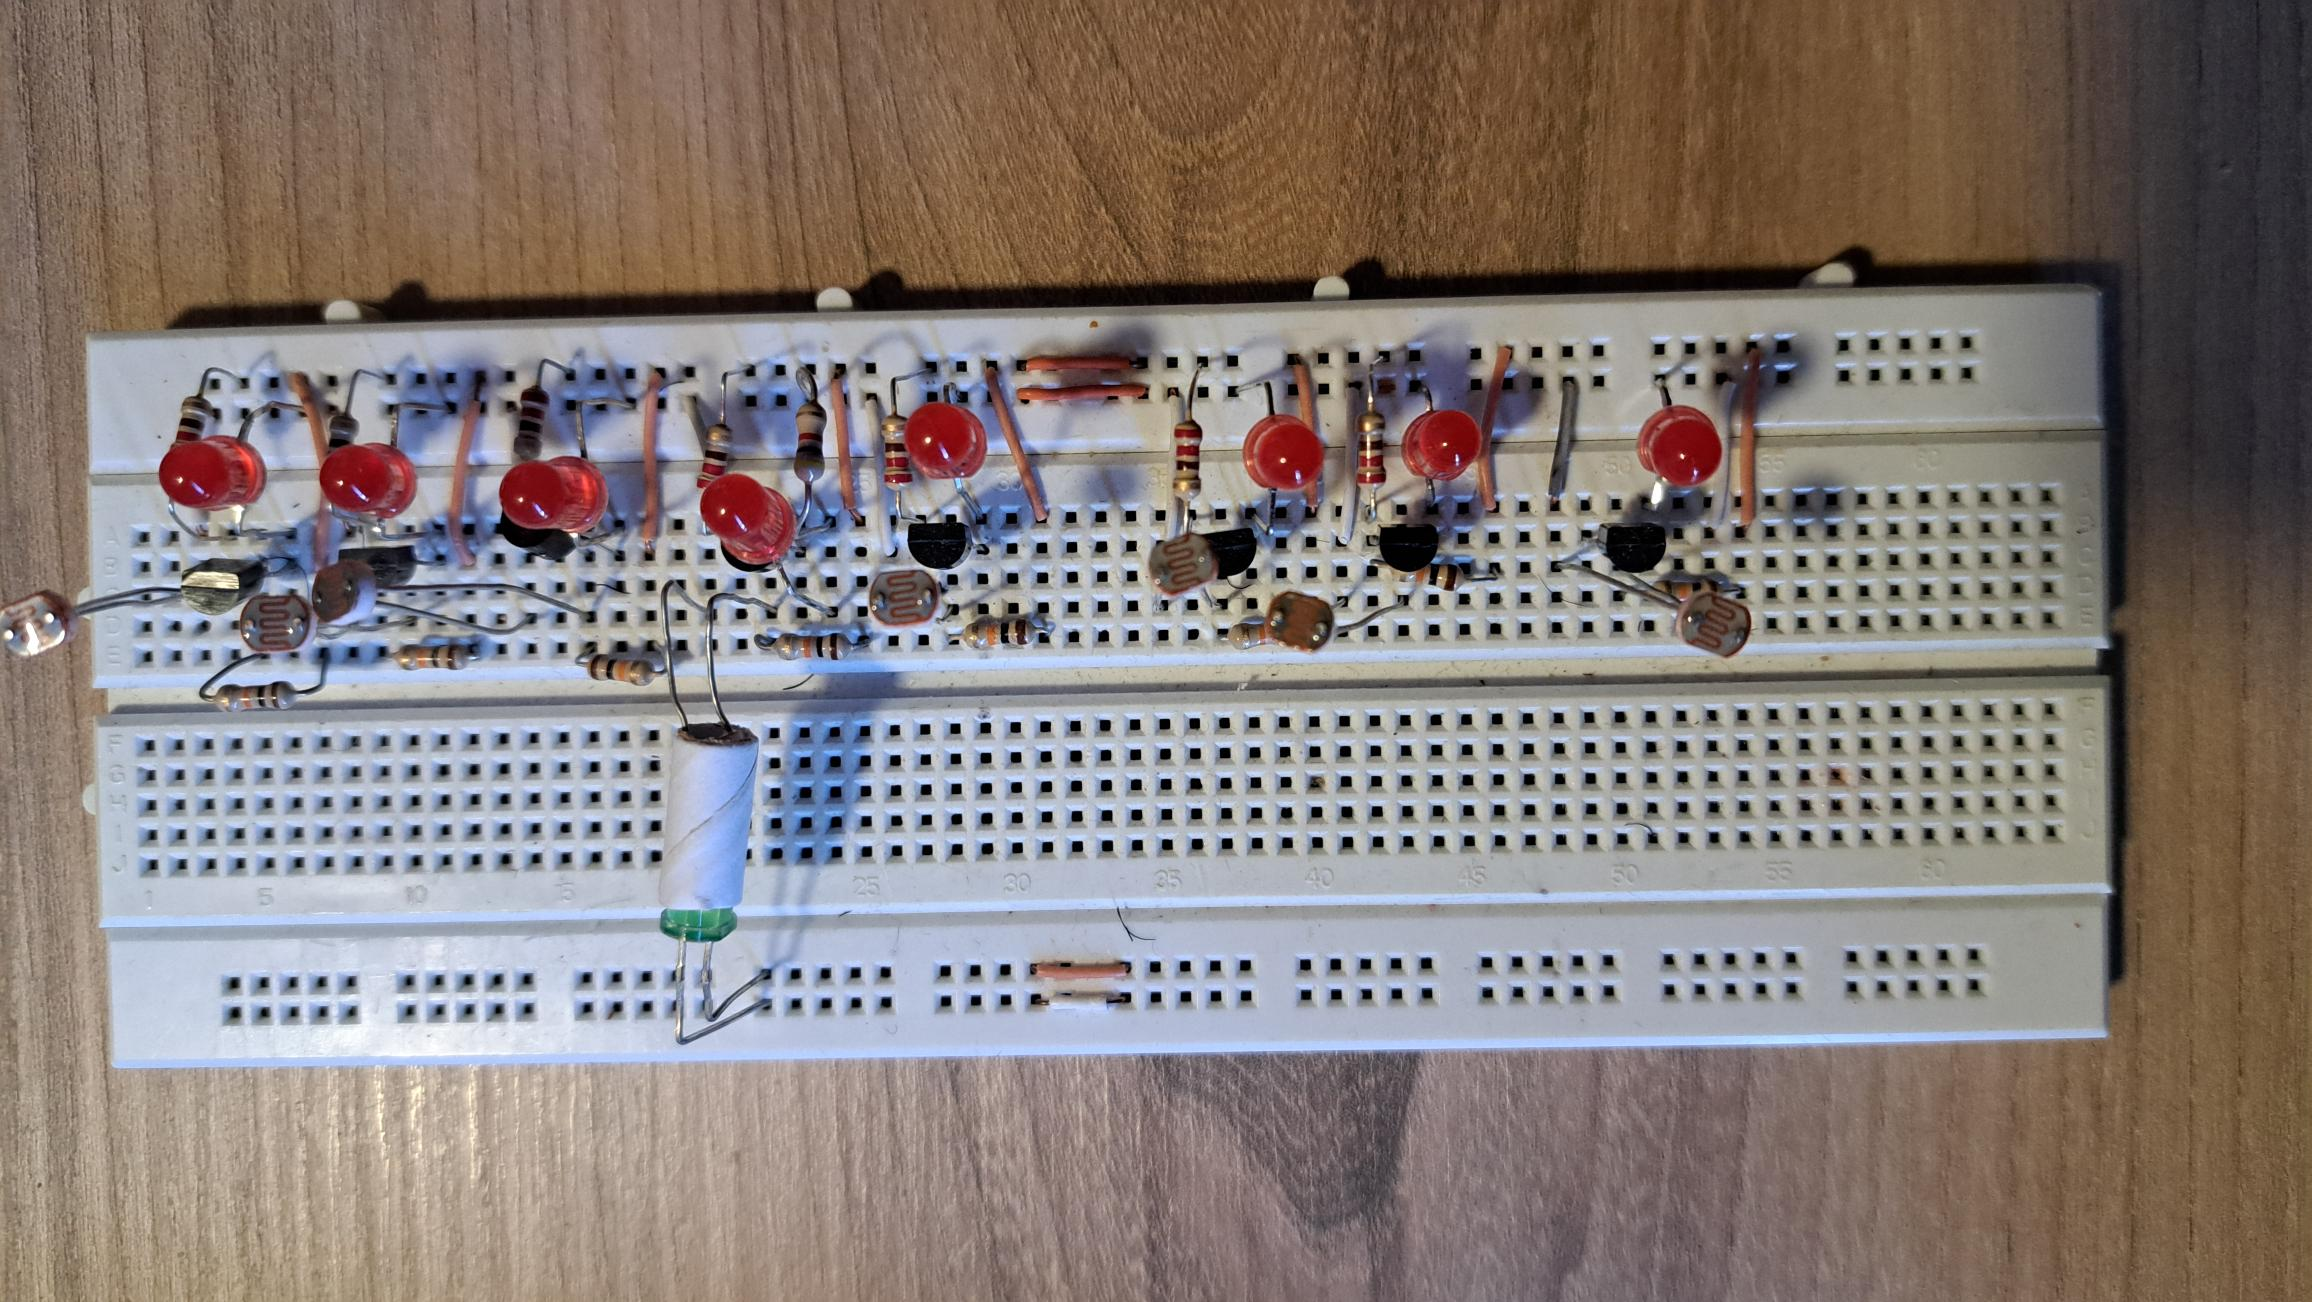
\includegraphics[width=0.45\linewidth]{body/ch6/figs/bread}
	\caption[Diagram of First Iteration of the Quantum Channel.]{Photograph image of QKD network model on a breadboard.}
	\label{fig:quantum-channel-bread}
\end{figure}
In the first iteration, a single fibre link was using to test the occlusive security measurements in place for prevent eavesdrop attacks. 

The second iteration was implemented on veroboard as illustrated in figure \ref{fig:veroboard}.
\begin{figure}[!ht]
	\centering
	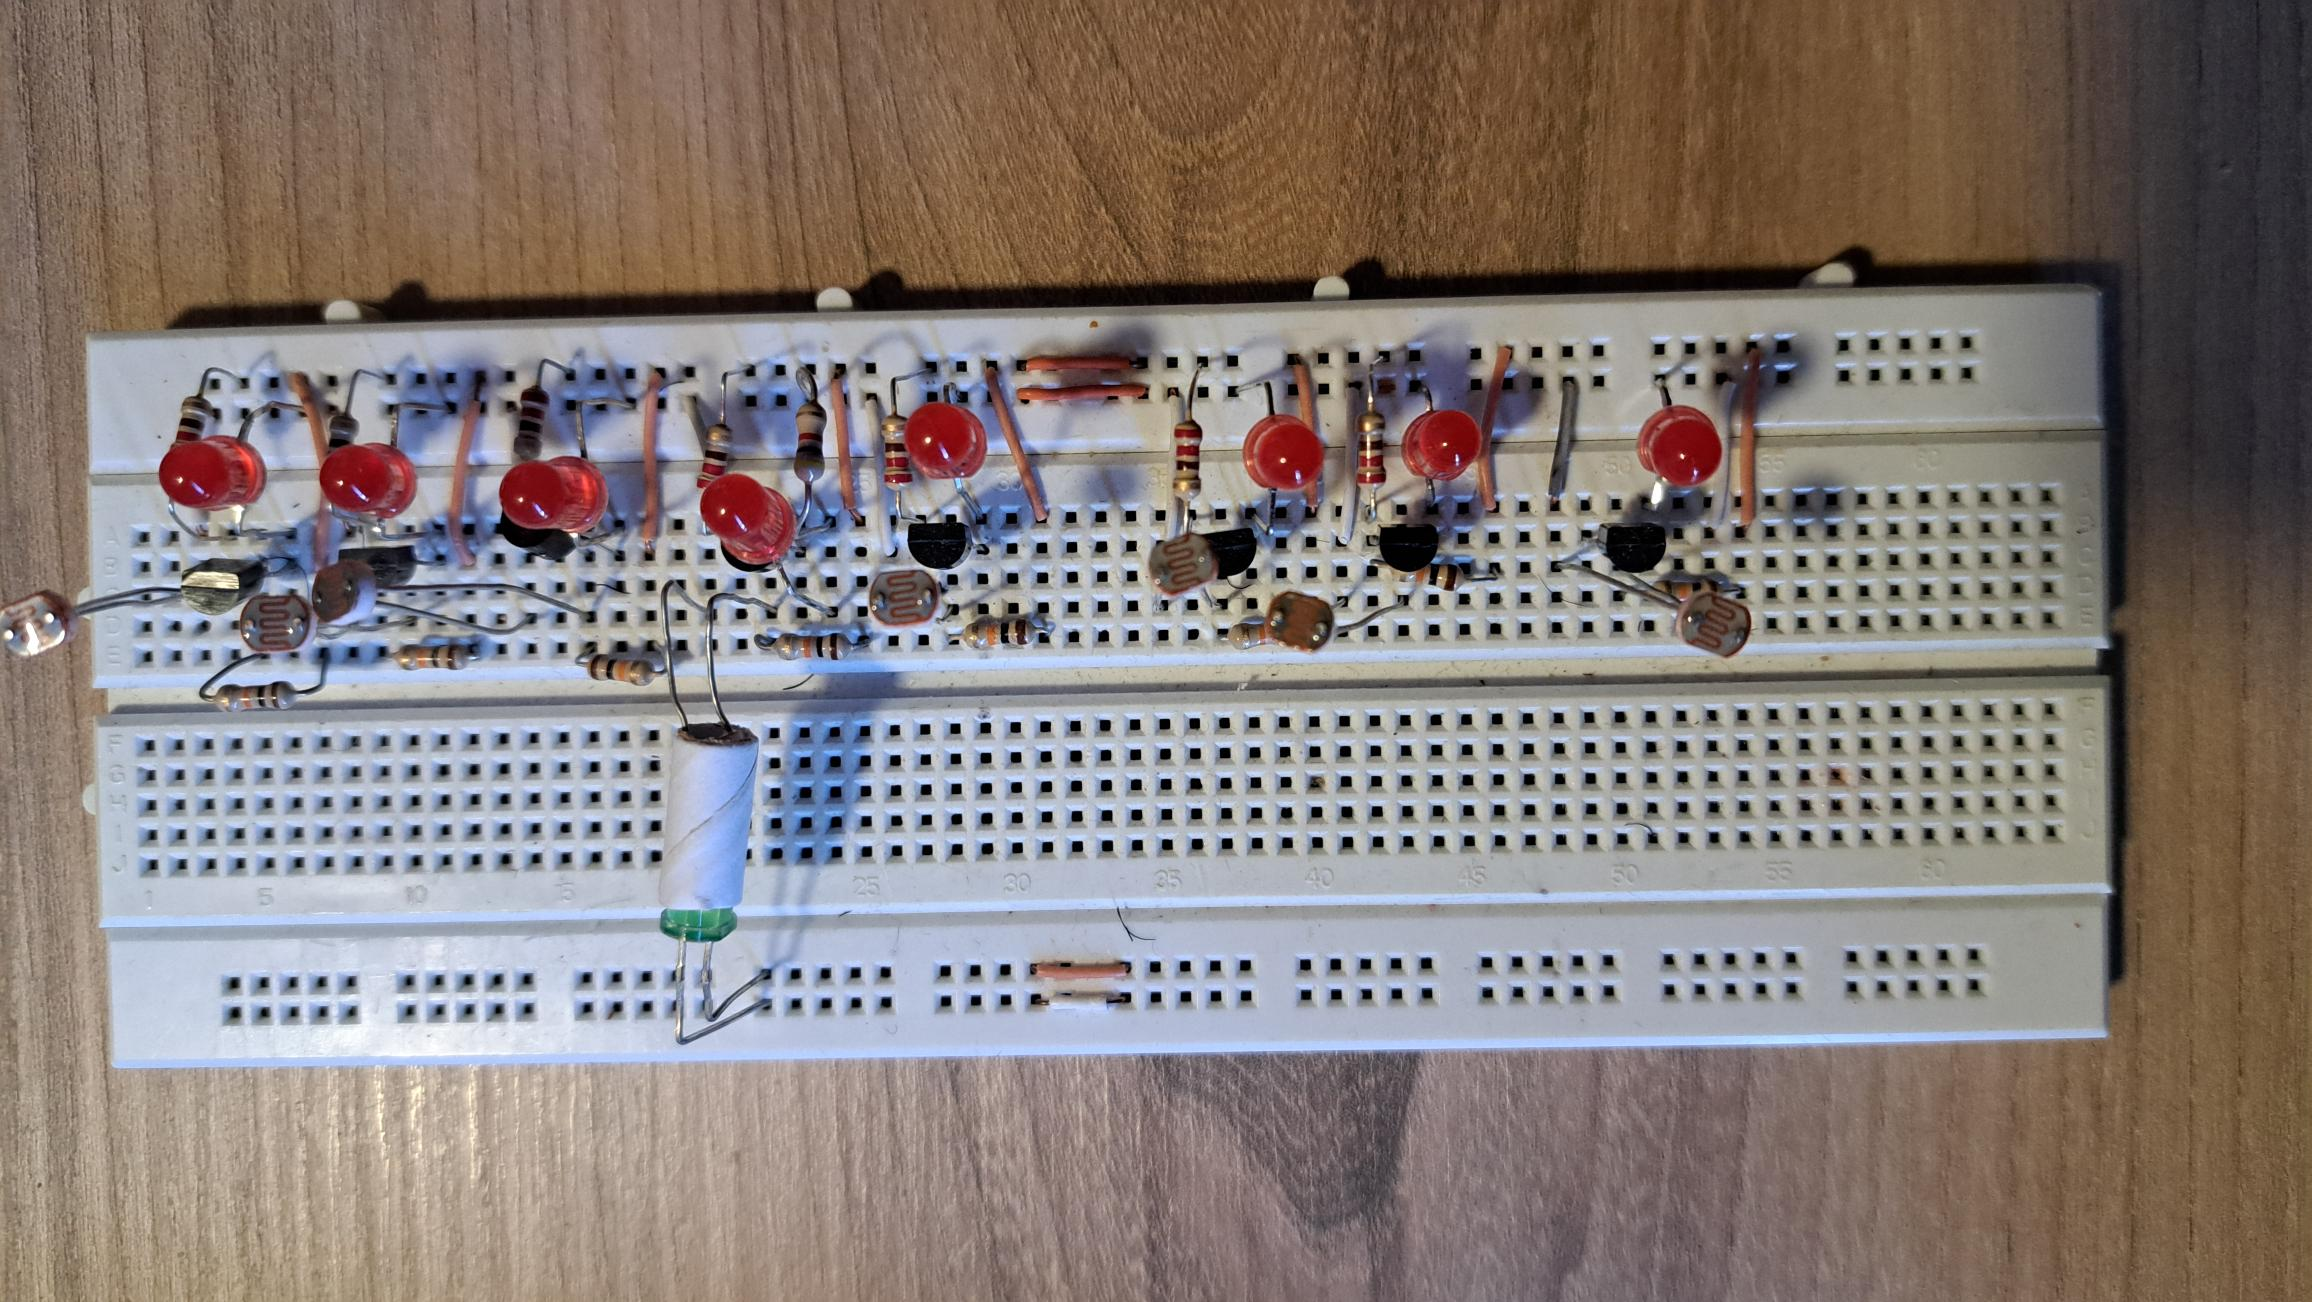
\includegraphics[width=0.45\linewidth]{body/ch6/figs/bread}
	\caption[Diagram of Second Iteration of the Quantum Channel On a Veroboard.]{Photograph image of QKD network model on a veroboard.}
	\label{fig:veroboard}
\end{figure}
The transmission requirements were met. However, due to the long bit patterns required for transmitting the Hilbert space, the transmission of qubits was restricted torrrrr


\subsubsection{Initialise Qubits on the STM32 Microcontroller Using Push-Buttons}

This \texttt{prepareEntangledPair} function was used during emulation of the quantum teleportation algorithm in which prior entanglement information was shared between Alice and Bob. When the microcontroller was reset or restarted, qubits returned to the separable ground state. 

\section{\label{sec:ch5_subsec1}Emulation of Quantum Teleportation Algorithm}

The quantum teleportation algorithm was successfully implemented on the Nexys-A7 FPGA. Results from the implementation of the quantum teleportation algorithm are listed in the figures below.

\begin{figure}[!ht]
	\centering
	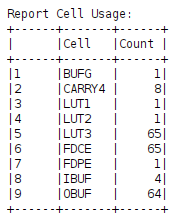
\includegraphics[width=0.45\linewidth]{body/ch6/figs/qta-resources}
	\caption[Showing Results from Synthesis of the Quantum Teleportation Algorithm]{Showing cell usage for synthesising the quantum teleportation algorithm using SystemVerilog in AMD Vivado.}
	\label{fig:qta-1}
\end{figure}

\begin{figure}[!ht]
	\centering
	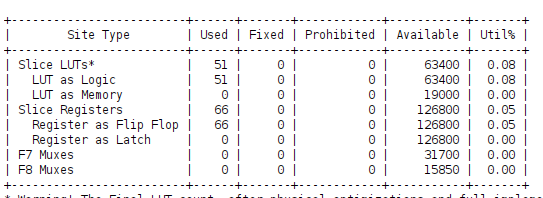
\includegraphics[width=0.45\linewidth]{body/ch6/figs/qta-resources-full}
	\caption[Showing Results from Synthesis of the Quantum Teleportation Algorithm]{Showing full cell usage for synthesising the quantum teleportation algorithm using SystemVerilog in AMD Vivado.}
\label{fig:qta-2}
\end{figure}

\begin{figure}[!ht]
	\centering
	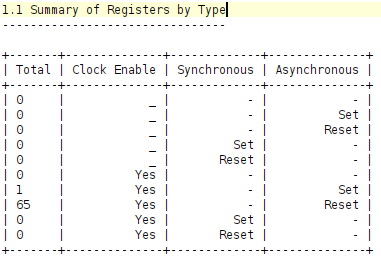
\includegraphics[width=0.45\linewidth]{body/ch6/figs/qta-registers}
	\caption[Showing Results from Synthesis of the Quantum Teleportation Algorithm]{Showing register usage during synthesis of the quantum teleportation algorithm using SystemVerilog in AMD Vivado.}
\label{fig:qta-3}
\end{figure}

\begin{figure}[!ht]
	\centering
	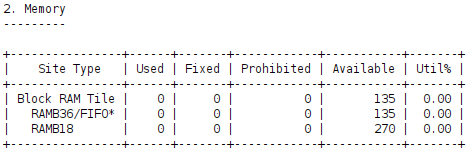
\includegraphics[width=0.45\linewidth]{body/ch6/figs/qta-memory}
	\caption[Showing Results from Synthesis of the Quantum Teleportation Algorithm]{Showing memory usage during synthesis of the quantum teleportation algorithm using SystemVerilog in AMD Vivado.}
\label{fig:qta-4}
\end{figure}

\begin{figure}[!ht]
	\centering
	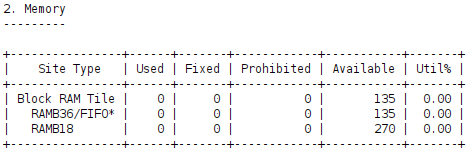
\includegraphics[width=0.45\linewidth]{body/ch6/figs/qta-memory}
	\caption[Showing Results from Synthesis of the Quantum Teleportation Algorithm]{Showing memory usage during synthesis of the quantum teleportation algorithm using SystemVerilog in AMD Vivado.}
\label{fig:qta-5}
\end{figure}

\subsubsection{Emulating the Quantum Fourier Transform}

In the initial attempt to convert the MATLAB description of the QFT quantum circuit to SystemVerilog, HDL Coder returned conformance errors related to the implementation of the \textit{tensor\_product} and \\texttt{controlled\_phase\_shift} functions. This is because when generating HDL code, dynamic-sized matrix variables are not allowed. To fix the errors, quantum gates operations were described in an element-wise manner with hard coded matrix sizes as illustrated in listing \ref{lst:qft-elementwise} corresponding to the first time step in the quantum circuit.
\begin{lstlisting}[language=Matlab, caption={MATLAB code fix for applying the tensor product function in using a method that conforms with HDL Coder.}, label={lst:qft-elementwise}]
% Initialise AB matrix for H ox I (4x4 matrix)
AB = complex(zeros(4, 4));

% Manually expand the tensor product
AB(1:2, 1:2) = H(1,1) * I;
AB(1:2, 3:4) = H(1,2) * I;
AB(3:4, 1:2) = H(2,1) * I;
AB(3:4, 3:4) = H(2,2) * I;

% Initialise result matrix for, 
% which results in an 8x8 matrix
result = complex(zeros(8, 8));

% Manually expand the tensor product 
result(1:2, 1:2) = AB(1,1) * I;
result(1:2, 3:4) = AB(1,2) * I;
result(1:2, 5:6) = AB(1,3) * I;
result(1:2, 7:8) = AB(1,4) * I;

result(3:4, 1:2) = AB(2,1) * I;
result(3:4, 3:4) = AB(2,2) * I;
result(3:4, 5:6) = AB(2,3) * I;
result(3:4, 7:8) = AB(2,4) * I;

result(5:6, 1:2) = AB(3,1) * I;
result(5:6, 3:4) = AB(3,2) * I;
result(5:6, 5:6) = AB(3,3) * I;
result(5:6, 7:8) = AB(3,4) * I;

result(7:8, 1:2) = AB(4,1) * I;
result(7:8, 3:4) = AB(4,2) * I;
result(7:8, 5:6) = AB(4,3) * I;
result(7:8, 7:8) = AB(4,4) * I;

H1 = result;
state_after_first_time_step = matrix_multiply(H1, initial_state);
\end{lstlisting} 
Expanding the high-level description of the QFT algorithm resulted in 695 lines of code for the execution of the full quantum circuit. Using HDL Coder, the MATLAB description was converted to the \textit{qft\_3qubit\_fixpt} SystemVerilog module as shown in the code snippet in \ref{lst:qft-sv}. The SystemVerilog code section shown directly relates to the element-wise operation in MATLAB as shown in listing \ref{lst:qft-elementwise}. The initial state variable was set to a \texttt{double(8x1)} corresponding to the 8 entries of the matrix representing the quantum register $\ket{q_0 q_1 q_2}$. In the first attempt of code generation, a fixed-point scheme number scheme with 14-bit signed words and 14-bit mantissas was used. 

\begin{lstlisting}[language=Verilog, caption={SystemVerilog code snippet for the QFT algorithm as generated by MATLAB HDL Coder corresponding to the description in \ref{lst:qft-elementwise}.}, label={lst:qft-sv}]
for(qft_3qubit_fixpt_t_1 = 32'sd0; ...
	qft_3qubit_fixpt_t_1 <= 32'sd1;
	qft_3qubit_fixpt_t_1 = qft_3qubit_fixpt_t_1 + 32'sd1) 
	begin
	for(qft_3qubit_fixpt_t_0 = 32'sd0;
	qft_3qubit_fixpt_t_0 <= 32'sd1;
	qft_3qubit_fixpt_t_0 = qft_3qubit_fixpt_t_0 + 32'sd1)...
	begin
	qft_3qubit_fixpt_add_cast[qft_3qubit_fixpt_t_0] ...
		= {{31{qft_3qubit_fixpt_t_1[31]}},...
		{qft_3qubit_fixpt_t_1, 1'b0}};
	qft_3qubit_fixpt_t_17 = nc[qft_3qubit_fixpt_t_0 ...
		+qft_3qubit_fixpt_add_cast[qft_3qubit_fixpt_t_0]];
	qft_3qubit_fixpt_add_cast_0[qft_3qubit_fixpt_t_0] ...
		= {{30{qft_3qubit_fixpt_t_1[31]}}, ...
		{qft_3qubit_fixpt_t_1, 2'b00}};
	qft_3qubit_fixpt_AB_re[qft_3qubit_fixpt_t_0 ...
		+ qft_3qubit_fixpt_add_cast_0[qft_3qubit_fixpt_t_0]] ...
		= qft_3qubit_fixpt_t_17;
	qft_3qubit_fixpt_add_cast_1[qft_3qubit_fixpt_t_0] ...
		= {{30{qft_3qubit_fixpt_t_1[31]}}, ... 
			{qft_3qubit_fixpt_t_1, 2'b00}};
	qft_3qubit_fixpt_AB_im[qft_3qubit_fixpt_t_0 + ...
	 qft_3qubit_fixpt_add_cast_1[qft_3qubit_fixpt_t_0]] = ...
	  14'sb00000000000000;
	qft_3qubit_fixpt_AB_re[qft_3qubit_fixpt_t_0 ...
	 + (32'sd4 * (32'sd2 + qft_3qubit_fixpt_t_1))] ...
	 = qft_3qubit_fixpt_t_17;
	qft_3qubit_fixpt_AB_im[qft_3qubit_fixpt_t_0 + ...
	 (32'sd4 * (32'sd2 + qft_3qubit_fixpt_t_1))] = ...
	 14'sb00000000000000;
	qft_3qubit_fixpt_add_cast_2[qft_3qubit_fixpt_t_0] ...
		= {{30{qft_3qubit_fixpt_t_1[31]}}, ... 
			{qft_3qubit_fixpt_t_1, 2'b00}};
	qft_3qubit_fixpt_AB_re[(qft_3qubit_fixpt_t_0 ...
		+ qft_3qubit_fixpt_add_cast_2[qft_3qubit_fixpt_t_0]) ...
		+ 32'sd2] = qft_3qubit_fixpt_t_17;
	qft_3qubit_fixpt_add_cast_4[qft_3qubit_fixpt_t_0] ...
		= {{30{qft_3qubit_fixpt_t_1[31]}}, ...
			{qft_3qubit_fixpt_t_1, 2'b00}};
	qft_3qubit_fixpt_AB_im[(qft_3qubit_fixpt_t_0 ...
		+ qft_3qubit_fixpt_add_cast_4[qft_3qubit_fixpt_t_0]) ...
		+ 32'sd2] = 14'sb00000000000000;
	qft_3qubit_fixpt_add_cast_6[qft_3qubit_fixpt_t_0] ...
		= {{31{qft_3qubit_fixpt_t_1[31]}}, ...
			 {qft_3qubit_fixpt_t_1, 1'b0}};
	qft_3qubit_fixpt_AB_re[(qft_3qubit_fixpt_t_0 ...
		+ (32'sd4 * (32'sd2 + qft_3qubit_fixpt_t_1))) ...
		+ 32'sd2] = nc_0[qft_3qubit_fixpt_t_0  ...
		+ qft_3qubit_fixpt_add_cast_6[qft_3qubit_fixpt_t_0]];
	qft_3qubit_fixpt_AB_im[(qft_3qubit_fixpt_t_0 ...
		+ (32'sd4 * (32'sd2 + qft_3qubit_fixpt_t_1))) ...
		+ 32'sd2] = 14'sb00000000000000;
	end
end
\end{lstlisting}
The HDL Resource Utilization Report of the \texttt{qft\_3qubit\_fixpt} SystemVerilog module output is summarised in the table in figure \ref{fig:qft-hdl-res-report}. The table shows that the design uses 640 14x14-bit multipliers. The large number multipliers was due to the element-wise operations involved in the MATLAB description. The dense matrix operations of the QFT quantum circuit also led to a high usage of adders/subtractors. The design required 812 32x64-bit adders, 480 32x32-bit adders, 640 19x19-bit adders and 128 32x32-bit subtractors to make a total of 2060 adders/substractors.
\begin{figure}[!ht]
	\centering
	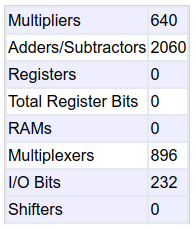
\includegraphics[width=0.45\linewidth]{body/ch6/figs/qft-hdl-res-report}
	\caption[Table Summarising the HDL Resource Utilisation Report in HDL Coder.]{Table summarising the HDL resource utilisation report in HDL Coder.}
	\label{fig:qft-hdl-res-report}
\end{figure}
The table also shows that 232 I/O bits were used in the design corresponding to 8 bits for the inputs and 112 bits for the real part of the final qubit Hilbert space and 112 bits for the complex part. This lead to an error during placement and routing because the Nexys-A7 target board uses a maximum of 210 I/O bits. To fix this issue, the design only considered the real part of the solution so that only 120 I/O bits could be used in total. 

The use of adders and multipliers was successfully modelled with Simulink as illustrated in figure \ref{fig:qft-simulink-1} corresponding to the initialisation of the qubit state in the first time step of the quantum circuit.
\begin{figure}[!ht]
	\centering
	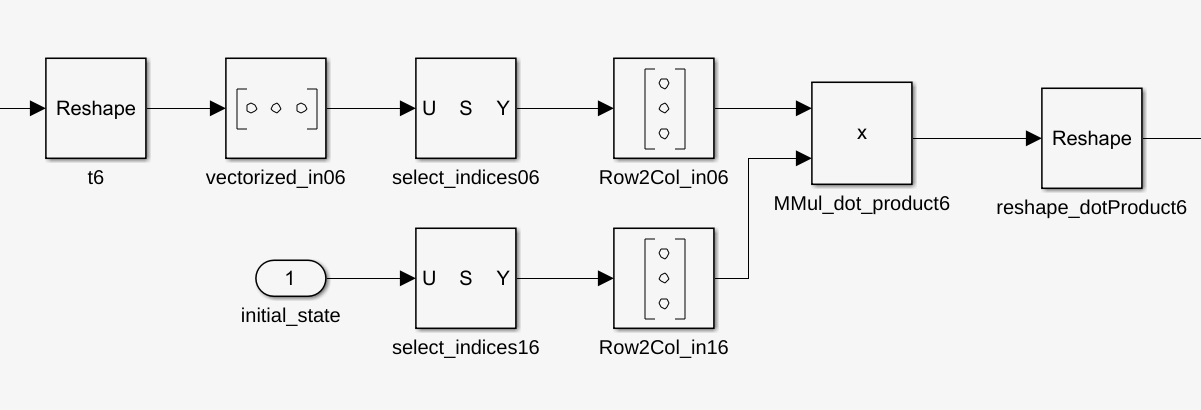
\includegraphics[width=\linewidth]{body/ch6/figs/qft-simulink-1}
	\caption[Initial Simulink Design Block for the QFT Quantum Circuit Described in MATLAB.]{Simulink initialisation of the $\ket{000}$ quantum state as a vector with 8 entries.}
	\label{fig:qft-simulink-1}
\end{figure}
In the result shown \ref{fig:qft-simulink-1}, it can be seen that no input register is used for the initial state. To improve the stability and signal integrity on each clock cycle, the design was altered to include a pipeline register for the input quantum state as shown by the green block in \ref{fig:qft-simulink-12}.
\begin{figure}[!ht]
	\centering
	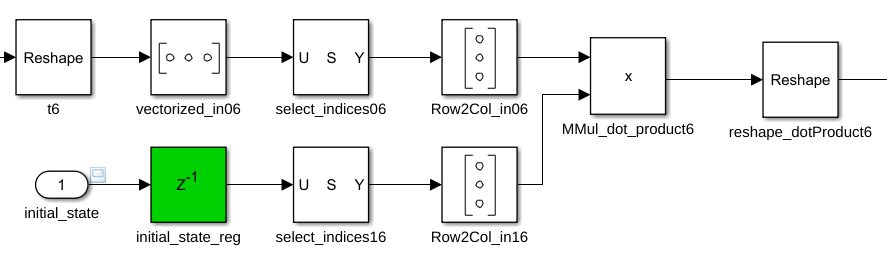
\includegraphics[width=\linewidth]{body/ch6/figs/qft-simulink-12}
	\caption[Showing the Simulink Model of the Input Quantum State with a Pipeline Register.]{The input register was used to stabilise the input signals for each clock cycle.}
	\label{fig:qft-simulink-12}
\end{figure}
The Simulink block design for the first time step of the QFT quantum circuit emulation is shown in figure \ref{fig:qft-first}. The result shows the multipliers, adders/subtractors and multiplexers described in the summary table in \ref{fig:qft-hdl-res-report}. The block diagram shows that 14 adders and selects to achieve a single quantum gate operation on a 3-qubit register.
\begin{figure}[!ht]
	\centering
	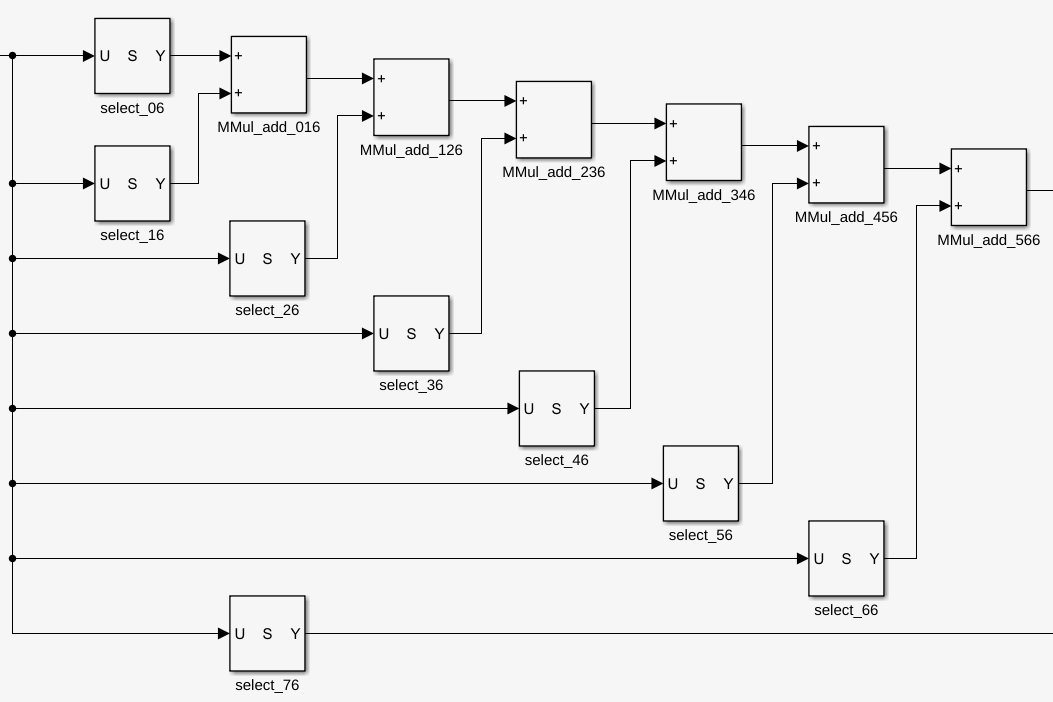
\includegraphics[width=\linewidth]{body/ch6/figs/qft-simulink-2}
	\caption[Showing the Simulink Model for Performing the First Time Step of the QFT Quantum Circuit where the Hadamard Gate is Applied to the Least Significant Qubit in the Quantum Register.]{Showing the simulink model for performing the first time step of the QFT quantum circuit where the \texttt{H} gate is applied to the LSQ in the quantum register as described in the design case study.}
	\label{fig:qft-first}
\end{figure}
Similarly, the output of the QFT was registered as shown in the snapshot of the Simulink block diagram in figure \ref{fig:qft-output-reg}. This allowed the qubits to be written synchronously at a rising edge.
\begin{figure}[!ht]
	\centering
	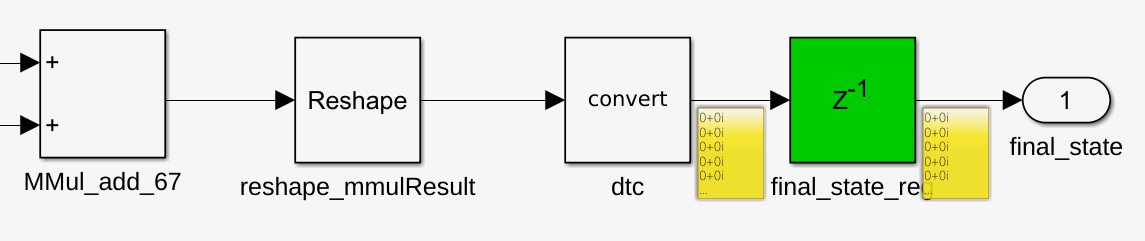
\includegraphics[width=\linewidth]{body/ch6/figs/qft-simulink-3}
	\caption[Showing the Output Register of the Quantum Fourier Transform in Simulink.]{An output pipeline register is used to hold the final QFT result to make it easier to interface with the UIS system.}
	\label{fig:qft-output-reg}
\end{figure}
After using registers and reducing the number of mantissas to 8 bits, the number of resources used in the QFT implementation was reduced significantly as shown in the summary table in figure \ref{tab:qft-summary-2}
\begin{figure}[!ht]
	\centering
	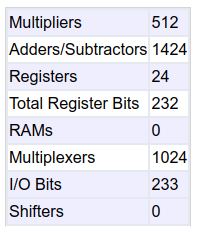
\includegraphics[width=0.55\linewidth]{body/ch6/figs/qft-summary-with-registers}
	\caption[Showing the HDL Coder Resource Utilisation Summary for the Pipelined QFT.]{Showing the HDL Coder resource utilisation summary for the pipelined QFT.}
	\label{fig:qft-summary-2}
\end{figure}
The summary shows that the number of 14x14-bit multipliers was reduced to 512. A more significant reduction was evident in the usage of adders/subtractors which was reduce from 2060 to 1424 in total. By reducing the number of mantissas to 8 bits, the highest reduction in the usage of resources was the 19x19-bit subtractors which were initially 640 and reduced to 192 in total.

The pipeline introduced 8 1-bit registers for storing the initial quantum state and 16 14-bit registers corresponding to the real and imaginary parts of each. The post synthesis report showed that out of 63400 available LUT slices, indicating that the design has a low resource footprint. The design also showed minimal usage of DSP slices. In total, only $10\%$ of the DSP slices available were utilised as shown in figure \ref{tab:qft-post-synth}. The pipeline introduced a data path delay of $\SI{19.869}{\nano\second}$. 

\begin{figure}[!ht]
	\centering
	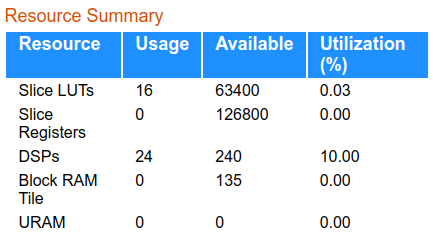
\includegraphics[width=0.45\linewidth]{body/ch6/figs/qft-post-synth}
	\caption[Showing the HDL Coder Post Synthesis Resource Summary.]{Showing the HDL Coder post synthesis resource utilisation summary for the pipelined QFT.}
	\label{fig:qft-post-synth}
\end{figure}

\subsection{Emulation of the Quantum Search Algorithm}

The quantum search algorithm was successfully emulated using a similar design procedure where HDL Coder was used to generated SystemVerilog modules and testbenches. The implementation used a 14-bit word with a 14-bit mantissa.  
%This section describes some results. This is how you can reference an appendix Appendix~\ref{app:sec:myappendix} as you might want to offload stuff to the appendix.

%Here is an example table

%\begin{table}[!ht]
%	\centering
%	\caption{Caption for table}
%	\begin{tabular}{l|l}
%		\hline
%		\textbf{Parameter}      & \textbf{Value}   \\ \hline
%		Lower cutoff frequency  & 100 kHz  \\
%		Mid frequency           & 200 kHz \\
%		Higher cutoff frequency & 300 kHz \\ \hline
%	\end{tabular}
%	\label{tb:mytablename}
%\end{table}
